\documentclass[acmsmall,nonacm,screen,review]{acmart}
\newif\ifEnableExtend
%\EnableExtendtrue
\EnableExtendfalse

\usepackage[utf8]{inputenc}
\usepackage{url}
\usepackage{color}
\newcommand{\csch}[1]{{\color{red} Christian says: #1}}
\newcommand{\Is}       {:=}
\newcommand{\set}[1]{\left\{ #1\right\}}
\newcommand{\sodass}{\,:\,}
\newcommand{\setGilt}[2]{\left\{ #1\sodass #2\right\}}
\usepackage{amsmath}
\usepackage{amsthm}
\usepackage{xspace}
\usepackage{relsize}

\usepackage{subcaption}
\usepackage{graphicx}

\newtheorem{openproblem}{Open Problem}
\newcommand{\ie}{i.\,e.,\xspace}
\newcommand{\eg}{e.\,g.,\xspace}
\newcommand{\etal}{et~al.\xspace}
\newcommand{\cov}{\term{cov}\xspace}
\newcommand{\term}[1]{\textsl{#1}}
\newcommand{\Comment}[1]{\textsl{#1}}

\def\MdR{\ensuremath{\mathbb{R}}}
\def\MdN{\ensuremath{\mathbb{N}}}

%%%%%%%%%%%%%%%%%%%%%%%%%%%%%
\setcopyright{none}
\copyrightyear{2023}
\acmYear{2023}
\acmDOI{}
\acmPrice{}
\acmISBN{}

\title{Flow-Partitioning within Hierarchical Process Mapping}
\author{Erben Jakob}
\email{jakob.erben@stud.uni-heidelberg.de,Msc. Data & Computer Sience,3727893}
\affiliation{%
  \institution{Heidelberg University}
  \streetaddress{Im Neuenheimer Feld 205}
  \city{Heidelberg}
  \state{Baden-Württemberg}
  \country{Germany}
  \postcode{69120}
}


\date{15,03,2023}

\begin{document}

\begin{abstract}
As the amount of communication in large computations increases it is increasingly 
crucial to find good algorithms which output a distribution of the suppresses such that
communication costs are minimized. Especially if the cost of communications are irregular 
\cite{predari2021mpi}. Therefore, it is important to know the architecture of the used 
system in order to map the different computational blocks on to processors in such a way, 
that the total cost of communication is held as low as possible. 
In our work we propose an alternation to the multilevel approach  presented by Faraj et 
al. \cite{Far20}, which enables the flow oriented refinement method to be aware of
the architecture of the system and the associated communication costs. 
However, while an easy theoretical advantage of this method could be shown this could 
not be reproduced in different experiments. 
\end{abstract}
\maketitle

\section{Introduction}
The problem of efficiently performing a large computation with certain amounts of 
communication between different components can be viewed as two separate problems.
First one needs to form blocks of tasks, where each block is executed on the same processor,
this can be achieved by partitioning the computation graph. Secondly these blocks then need
to be mapped to physical processors in the system. This mapping needs to be considerate of 
the architecture of the system, as any two processors may either bee in identical areas 
(i.e. they have a small distance) or they are far away from one another (i.e. they have a 
large distance). As recent research \cite{berti2006mpi} however showed that an overall 
improvement in performance can be reached when both tasks not performed separately but 
aware of one another. The approach requires two make two assumptions about modern 
supercomputer systems which are generally valid. Firstly that communication patterns are
sparse and secondly that there is a hierarchical representation of those patterns. In this 
hierarchical representation two nodes of the same level always have the same speed of 
communication. On this basis the multilevel approach was developed, which improved the process
mapping task by integrating it into highly performant multilevel partitioning algorithms. 
The multilevel approach contracts the problem to a smaller problem and then can use partitioning
algorithms to solve these compacted versions. One of the possible partitioning algorithms it 
uses is a flow partitioner which relies on a result from graph theory, that shows that the size 
of a minimum cut equals the size of a maximum flow. Hence, one can find a minimum cut, by 
determining the maximum flow.

\section{Preliminaries}
\subsection{Basic Concepts}
\label{subsec:basic_concepts}
Let $G=(V=\{0,\ldots, n-1\},E)$ be an \emph{undirected graph} with edge weights $\omega: 
E \to \MdR_{>0}$, vertex weights $c: V \to \MdR_{\geq 0}$, $n = |V|$, and $m = |E|$.

The \emph{graph partitioning problem} is concerned with partitioning all $v in V$ into k distinct 
subsets called blocks, a solution which uses k blocks is called a k-partition. The quality of a 
solution is determined by the size of the created edge cut as well as the balance of the blocks. 
Let us denote the blocks with $V_1$,\ldots,$V_k$. Note that by distinctiveness and completeness 
of the subsets, the following must hold: $V_1\cup\cdots\cup V_k=V$ and $V_i\cap V_j=\emptyset$ 
for $i\neq j$. The \emph{balancing constraint} ensures that the weight of a block (the sum of
weights of a blocks vertices) does not exceed a threshold respecting a balancing factor 
$\epsilon$. Hence, for $i \neq j: c(V_i)\leq c(V_j)*(1+\epsilon)$. The \emph{edge-cut} of a 
$k$-partition measures the weight of all edges incident to two vertices of different blocks. 
It can be expressed as $\sum_{i<j}\omega(E_{ij})$, where $E_{ij}\Is\setGilt{\set{u,v}\in E}
{u\in V_i,v\in V_j}$. 

For a k-partition we call a pair of blocks \emph{neighboring blocks} if they are connected by some edge.
Any node $v \in V_i$ which has a neighbor $w \in V_j, i\neq j$ is part of the boundary its block 
and is hence called \emph{boundary node}.

In order to perform a flow partitioning we need to change our representation of a graph slightly, by 
defining a corresponding network for which the problem can be solved. Therefore, let $G_f=(V_f,E_f)$
be a flow graph. Starting from a graph G we added two additional vertices called \emph{source} and 
\emph{train} (short: $s,t$) to the vertices (\ie$V'=V \cup \set{s,t}$). All edges are directed meaning
$e=(u,v)$ is an edge from vertex $u$ to vertex $v$ and each edge has a non-negative capacity assigned 
with it ($\ie cap(u,v)$). A flow function is a function on the edges of a network (which can now be 
interpreted as a tuple of vertices). A function $\setGilt{f}{V_f \times V_f \rightarrow\MdR_{>0}}$ is a
flow if it fulfills three constraints. It has to satisfie a \emph{capacity constraint} ($\ie f(u,v)\leq$),
a \emph{symmetric constraint} ($\ie f(u,v)=-f(v,u)$) and \emph{flow conservation constraint} in all 
vertices except $s$ and $t$ ($\ie \setGilt{\sum_{v\in N(u)}f(u,v)=0}{\forall v\in V' \backslash \set{s,t}}$).
Ford and Fulkerson showed in 1956 that the value of a flow $|f|=sum_{v\in V_f f(s,v)}$ if it is maximal 
($\ie |f|\geq|f'|$ for any st-flow $f'$) is identical to the weight of a minimal \emph{ST-cut}. A minimal
cut is a set of edges $S$ which separates $s$ from $t$, such a set is minimal if the sum of its edges
capacities is minimal.  

Assume that we are partitioning $n$ processes for a topology containing $k$ processing elements (PEs).
Let $\mathcal{C}\in \MdR^{n \times n}$ denote a matrix indicating the communication volumes and 
let $\mathcal{D}\in \MdR^{k \times k}$ denote the (implicit) topology matrix or distance matrix.
For two processes $i$ and $j$ the amount of communication between them is denoted with $\mathcal{C}_{i,j}$. 
Say they are assigned to PEs $x$ and $y$ then the distance matrix gives a cost per communication
between the two PEs $\mathcal{D}_{x,y}$. Therefore, the total cost of communication can be expressed as 
$\mathcal{C}_{i,j}\mathcal{D}_{x,y}$.
 
Based on the assumption, that supercomputers are hierarchically structured, the structure of the system
is described with a hierarchy sequence $\mathcal{S}=a_1: a_2: ...:a_\ell$. It indicates that each 
processor has $a_1$ cores, each node $a_2$ processors, each rack $a_3$ nodes, and so forth. 
$k=\Pi_{i=1}^{\ell}a_i$ hence expresses the total number of PE's in the system.
Similarly, $D = d_1:d_2:\ldots:d_\ell$ is a sequence which describes the communication cost 
between the different hierarchy levels. Two cores in the same processor communicate with cost 
$d_1$, two cores in the same node but in different processors communicate with cost $d_2$, two 
cores in the same rack but in different nodes communicate with cost $d_3$, and so forth.

\subsection{Related Work}
There has been a lot of work on problem of graph processing, for further information we refer to
\cite{bichot2013graph} \cite{bulucc2016recent} \cite{schulz2018graph}.
There have been different approaches to the task of process mapping in recent years. Kirchbach et al.
\cite{kirchbach2020better} tackled the problem by splitting the problem into a graph partitioning 
a subsequent mapping of said partitions onto the different PEs. However, it was shown that by Berti 
and Träff \cite{berti2006mpi}, that such a division of the tasks could lead to worse results.

M. F. Faraj, A. van der Grinten, H. Meyerhenke et al. \cite{Far20} extended the multilevel 
graph partitioner to also be able to solve the process mapping problem. They therefore could 
consider both the partitioning and the mapping at the same time, as well as make use of the good 
results of the multilevel partitioner.

Predari, Tzovas, Schulz et al. \cite{predari2021mpi} used an MPI-based algorithm, to solve the
process mapping issue in a parallelized fashion. It combines the parallel partitioner ParHIP and 
parallel label propagation mapping in order to receive, to get a fast but still relatively high 
quality process mapping solution.

The flow partitioning uses the equality of the size of a minimum cut and s maximum flow for proof
of this equality we refer the reader to \cite{diestel2017flows}. For an efficient implementation
of the push relabel algorithm we want to point to \cite{cherkassky1997implementing} as well 
as the paper introducing the algorithm \cite{goldberg1988new}. 

\section{Distance-aware flow partitioning}
We will proceed this explanation in three steps. Firstly the general flow partitioning approach is
described, secondly a theoretical example is shown for which the communication unaware version 
performs poorly. Lastly the extension, which enables the consideration of the explicit communication
costs, is explained. The flow partitioner is used during refinement the multilevel algorithm 
has already computed a partition and after the uncontraction the quality of the solution is refined.

\subsection*{Flow partitioner}
Call the two already existing partitions $L$ and $R$ we can construct the network for computing the 
flows as follows: $V_f = L \cup R \cup{s,t}$ and $E_f = E_{L,R} \cup \setGilt{sl}{s,l \in L} \cup 
\setGilt{rt}{r \in R, t}$ where $E_{L,R}$ is the set of edged between the nodes in $L$ and $R$.
Please note that all edges connecting some vertex to either s or t are assigned infinite capacity,
such that they are never fully saturated and hence can never be part of a minimal st-cut. 
A St-cut in this network would give a partition of the nodes of the nodes into $L'$ (all vertices 
reachable from s) and $R'$ such that the edge cut minimal if it is identical to the maximum flow.
The overall process would now work as follows: Take two given partitions and create a network. 
Secondly compute a maximum flow. This could be done with a few different algorithms, the given 
implementation uses the \emph{Push-Relabel algorithm} to find the maximum flow. After the maximal
flow was determined, a set of edges with same sum of weights can be found and the one which minimizes 
the cut while giving the best balance is returned. While this approach has been used successfully 
used in graph partitioning it can run into issues for process mapping as the next example will show. 

\subsection*{Example problem distance unaware partitioner}
This version of a flow partitioner has however one shortcoming, as it is not aware of the distances
between PEs. Lets for example assume there are 4 partitions and corresponding PEs (A, B, C and D). 
Let's assume all edges between individual tasks in the graph have the same amount of communication 
and hence a weight of one. Say $e(A,B)$ is the number of edges between partition A and B and as all
edges have weight one this is identical to the amount of communication (not considering distance) 
between any two $\sum_{ a \in A, b \in B}\mathcal{C}_{i,j}=\sum_{\setGilt{a \in A,b \in B}
{(a,b)=e}}\omega(e)$.

Now assume that $e(A,B) = e(A,C) = e(B,C) = 3$ and that $\mathcal{D}_{A,B}$ = $\mathcal{D}_{A,C}$ = 1 
and that $\mathcal{D}_{B,C}=10$. This configuration gives a cost total communication cost of 
$e(B,C)*\mathcal{D}_{B,C}+e(A,B)*\mathcal{D}_{A,B}+e(A,C)*\mathcal{D}_{A,C}=3*10+3*1+3*1=36$. 
Assume now that the flow partitioner moves two vertices from $A$ to $B$ giving $A'$ and $B'$ and 
with $e(A',B')=1$. Then it initially seems like the partitioner decreased the total amount of 
communication by two. However, further assume that one of the moved vertices was also connected to C. 
Hence get $e(A',B')=1, e(A',C)=2$ and $e(B',C)=4$. With the same distances as before this 
gives a total cost of $e(B',C)*\mathcal{D}_{B,C}+e(A',B')*\mathcal{D}_{A,B}+e(A',C)*\mathcal{D}_{A,C}=
4*10+1*1+2*1=43$ and the total cost has actually increased to by seven.

\subsection*{Distance aware partitioner}
To avoid these cases this work introduces a version of the flow partitioner which is aware of the actual
cost of moving vertices in between partitions. This is archived by two modifications to the network model.
Firstly the capacity function $\omega$ is modified to also consider the distance between the two 
partitions under consideration. Secondly additional edges are introduced to consider the true change in 
communication cost when moving a vertex in between partitions.

To make the actual communication cost more pronounced we multiply all capacities of edges not incident to
s or t, with the distance between the two PEs associated with partitions under consideration. Assume again
that all weights are 1 and that $\mathcal{D}_{A,B} = 3$. Then a minimal cut with three edges would have an 
accurate weight of nine. Please note that this change alone will not change the outputs of the flow problem
as it scales all edge weights uniformly and hence simply scales the problem itself.

To correctly consider the change in communication cost when partitioning we introduce two additional edges 
for each vertex ($\neq s,t$). One of which goes from s to any vertex and one which goes from that vertex to
t. These edges encode 2 different information depending on the original position of the vertex. Let's look
at any $l\in L$ then the edge from it to $t$ encodes the current cost of communication to vertices not in
part of the considered partitions. Hence, if the algorithm decided to cut this edge then l would be part 
of $L_{new}$ then the cost of cutting this edge would represent the communication associated with the outside
communication with l. Similarly, for some vertex $r \in R$ the same information about the current communication
cost is represented in an edge to s. All vertices have a second edge encoding the potential cost with moving
the vertex to the other side for all $l \ in L$ those edges start in s, and for all $r \in R$ they end in t.
Say the algorithm decides to cut one of those edges for a left vertex then this resembles the outside information
associated with a partitioning where l is part of R'. There are two sets of newly created edges are called
\emph{communication correction edges drain} (CCD) and \emph{communication correction edges source} (CCS).
The weight of these edges can be described as follows:
$$\text{CCS: }\forall l \in L : cap(s,l) = \sum_{x\in N(l)\backslash\{L\cup R\}}\mathcal{D}_{R,pe(x)}*\mathcal{C}_{l,x}$$
$$\text{CCD: }\forall l \in L : cap(l,t) = \sum_{x\in N(l)\backslash\{L\cup R\}}\mathcal{D}_{L,pe(x)}*\mathcal{C}_{l,x}$$
Similarily, the weights can be defined for edges adjacent to the right partition.

Going back to the example from the last subsection it is impossible for the distance aware flow partitioner 
to move vertices in a way such that the total weight of communication increases instead of decreasing, as 
it processes all needed information to avoid these mistakes.

\section{Experiments}
We implemented our work within the MultiLevelMap Framework (C++) which is based on the KaHIP framework. We compiled the project
with compiler version [MISSING] and the following optimization settings [Missing]. The used machine was running Ubuntu
22.04 and the kernel version 5.19.0-32. It contained an 8-core / 16-thread Ryzen 7 5825U processor clocked at up to 4.5 GHz and 
was equipped with a total of 16 gigabytes of RAM. All tests allowed for a total of 3\% of imbalance and were tested for different
partition counts. These depended on the hierarchy describing sequence the following sequences were used.
Let the set of test-sequences be $S' = \setGilt{\set{4:16:64*k}}{k \in \set{1,2,4,8,16,32,64,128}}$. This resulted in three different
hierarchical levels which were assigned the following distance sequence $D = \set{1:10:100}$. Lastly a fixed seed was used in order to keep
results as reproducible as possible.

\subsection{Dataset}
The graphs for testing the algorithm come from two sources. Firstly the five largest
graphs from Chris Walshaw's benchmark archive \cite{soper2004combined} were used. 
All further graphs were originally part of the 10th DIMACS Implementation
Challenge \cite{benchmarksfornetworksanalysis}. All $rgg_X$ are random geometric graphs with
$2^X$ nodes. Each node can be interpreted as a random point in the unit square two nodes are connected
if the Euclidean distance between them is below 0.55 $\frac{ln(n)}{n}$. The graphs $del_X$ are so-called
Delaunay triangulation of $2^x$ random points in the unit square. There are some graphs form the numerical
graph section of the DIMACS benchmark set (i.e. af-shell9, af-shell10 ...). The graphs europe, asia, 
great-britain, belgium and germany are large road networks of the respective areas \cite{DSSW09}. 
Table \ref{tab:instances} shows the basic properties of the graphs that were used.
\begin{table}[ht]
  \begin{tabular}{ |p{3cm}|p{1.5cm}|p{1.5cm}|p{3cm}|p{1.5cm}|p{1.5cm}|  }
    \hline
    Graph-Instance & n & m & Graph-Instance & n & m\\
    \hline
    \hline
    \multicolumn{6}{|c|}{Walshaw instances} \\
    \hline
    auto & $\sim$450k & $\sim$3.3M & 144 & $\sim$145k & $\sim$1M\\
    bcsstk30 & $\sim$28k & $\sim$1M & bcsstk32 & $\sim$45k & $\sim$100k\\
    m14b & $\sim$215k & $\sim$1.6M &  &  & \\
    \hline
    \multicolumn{6}{|c|}{road-network instances} \\
    \hline
    asia & $\sim$12M & $\sim$13M & belgium & $\sim$1.4M & $\sim$1.5M\\
    europe & $\sim$2M & $\sim$6.5M & germany & $\sim$11.5M & $\sim$12M\\
    great-britain & $\sim$7.7M & $\sim$8.1M &  &  & \\
    \hline
    \multicolumn{6}{|c|}{numerical instances} \\
    \hline
    af-shell9 & $\sim$500k & $\sim$8.5M & af-shell10 & $\sim$1.5M & $\sim$25M\\
    audikw1 & $\sim$940k & $\sim$38M & ecology-1 & $\sim$1M & $\sim$2M\\
    ecology-2 & $\sim$1M & $\sim$2M & G3-circuit & $\sim$1.5M & $\sim$3M\\
    kkt-power & $\sim$2M & $\sim$6.5M & ldoor & $\sim$950k & $\sim$23M\\
    nlpkkt120 & $\sim$3.5M & $\sim$46M &  &  & \\
    \hline
    \multicolumn{6}{|c|}{delauny and random geometric instances} \\
    \hline
    delauny10 & $\sim$1M & $\sim$1.9M & delauny15 & $\sim$32k & $\sim$98k\\
    delauny24 & $\sim$16M & $\sim$50M & rgg15 & $\sim$32k & $\sim$160k\\
    rgg23 & $\sim$8.3M & $\sim$63M &  &  & \\
    \hline
    \multicolumn{6}{|c|}{various instances} \\
    \hline
    vsp-barth5 & $\sim$32k & $\sim$100k & vsp-beref & $\sim$14k & $\sim$98k\\
    citation & $\sim$270k & $\sim$1.1M & coAuthers &  $\sim$300k & $\sim$980k\\
    \hline
  \end{tabular}
  \caption{Tested graph-instances}
  \label{tab:instances}
\end{table}
\newpage
\subsection{Comparison against state of the art}
In a first experiment the results for the final objective between the standard algorithm used by 
MultiLevelMap and a version which uses a distance aware flow partitioner are compared. Image \ref{fig:comparison_vanilla_strong}
shows the percentile increase for the different k-values averaged over the different graphs for the
strong configuration of the MultiLevelMap algorithm. Image \ref{fig:comp_vanilla_social} shows the same result for the social
configuration. In both cases the distance aware flow partitioner performs worse than the standard Fibonacci-
Mathesis multiway partitioner. The results are about 3\% worse than the baseline.

\begin{figure}
  \captionsetup[subfigure]{justification=centering}
\centering
\begin{subfigure}[t]{0.485\textwidth}
  \centering
  \includegraphics[width=\textwidth]{images/perctentage_increase_finalobjective_strong_vanialla_vs_improved.png}
  \caption{Percentage increase in final objective-  - strong configuration}
  \label{fig:comparison_vanilla_strong}
\end{subfigure}
\begin{subfigure}[t]{0.485\textwidth}
  \centering
  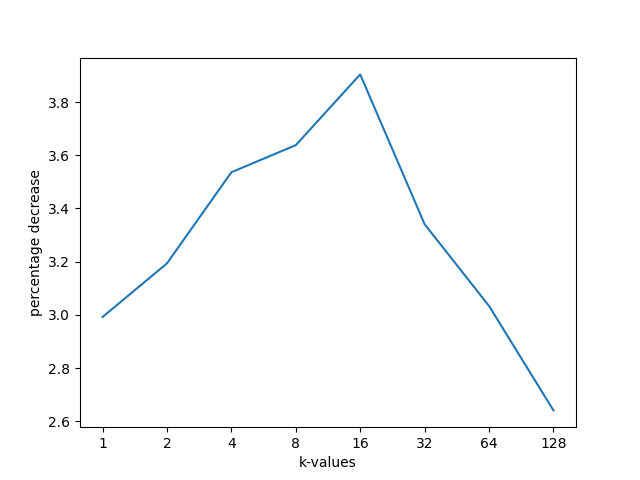
\includegraphics[width=\textwidth]{images/perctentage_increase_finalobjective_social_vanialla_vs_improved.png}
  %\vskip 0.1in
  \caption{Percentage increase in final objective-  - social configuration}
  \label{fig:comp_vanilla_social}
\end{subfigure}

\caption{Comparison distance aware flow partitioner vs. baseline implementation of MultiLevelMap}
\label{fig:LSeco}
\end{figure} 


\begin{figure}[b]
  \centering
  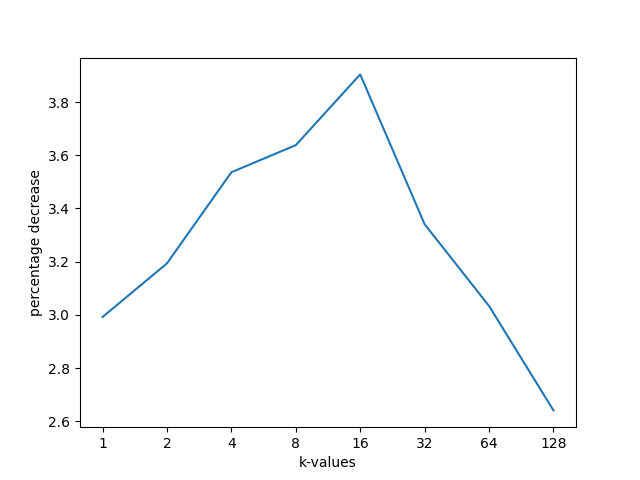
\includegraphics[width=0.485\textwidth]{images/perctentage_increase_finalobjective_social_vanialla_vs_improved.png}
  \caption{Percentage increase in final objective-  - social configuration}
  \label{fig:comp_flows}
\end{figure}

\subsection{Comparison against flow partitioner}
Additionally, the distance aware flow partitioner was compared against the standard version. Image \ref{fig:comp_flows} shows
the percentage decrease in the final objective value compared over all instances. One can see that it alternates
around 0\% which tells us two information. Firstly there are instances where the distance aware partitioner leads
to a better solution and hence its theoretical benefits can in some cases be used. Secondly it appears that
the MultiLevelMap algorithm produces good results regardless of distance awareness as the partition quality seems
to be deciding factor in the final objective score. 

\section{Conclusion}
While the distance aware flow partitioner seems like a good idea from a theoretical standpoint
it did not lead to a success in implementation as the experiments determined that it did not significantly
lead to better results than the standard flow partitioner, which meant that it could not replace 
the standard partitioning solution of the MultiLevelMap algorithm. Despite all of this it could be possible
that the distance aware flow partitioner could lead to improved results in some other configuration or 
some other problem, where a secondary factor determines the true result of a cut. 


\bibliographystyle{plainnat}
\bibliography{references.bib}

\end{document}